\documentclass{article}

\usepackage{fullpage}
\usepackage{enumerate}
\usepackage{tikz}
\usepackage{bm}

\title{CS181 Assignment 3: Clustering and Parameter Estimation}
\author{Lucas Freitas and Angela Li}
\date{\today}

\begin{document}
\maketitle

\section*{Problem 1}

\begin{enumerate}[a.]

\item % 1a

The probability $\rho = P(\max_m |x_m - y_m| \leq \epsilon)$ can be stated more simply as the probability that, for every dimension $m \in M$, $y_m$ is no more than $\epsilon$ away from $x_m$. So:

$$\displaystyle \rho = \prod_{m = 1}^{M} P(x_m - \epsilon \leq y_m \leq x_m + \epsilon)$$

Every $y_m$ is i.i.d. and uniformly distributed on $[0, 1]$, and for such a distribution the probability that a random variable takes on a value in some interval is the length of that interval. In this case, the length of $[x_m - \epsilon, x_m + \epsilon]$ is $2\epsilon$, thus: 

$$\rho = (2\epsilon)^M$$

\item % 1b

In part (a), every $x_m$ has a value of 0.5 (as $\bm{x}$ is the center of the unit hypercube), which is why the length of $[x_m - \epsilon, x_m + \epsilon]$ is always $2\epsilon$. However, if $\bm{x}$ can be any point in the unit hypercube, then any given $x_m$ may not necessarily be $\geq \epsilon$ away from 0 or 1, further constraining the desired interval for $y_m$ (and since, as mentioned before, the probability of $y_m$ falling in that interval is the length of the interval, that probability decreases). \\

That is, unlike in part (a), there is now a nonzero probability that $x_m - \epsilon < 0$ or $x_m + \epsilon > 1$, meaning the length of the interval in which $y_m$ should fall is smaller than the length of $[x_m - \epsilon, x_m + \epsilon]$. If this happens, there is a smaller $P(|x_m - y_m| \leq \epsilon)$ than $2\epsilon$, meaning the final probability is $\leq \rho$.

\item % 1c

The distance $||\bm{x} - \bm{y}||$ is equal to:

$$\sqrt{\sum_m (x_m - y_m)^2}$$

Assume that all for all $m$ save for one, $x_m = y_m$. The value of $\max_m |x_m - y_m|$ is the difference between those two coordinates where $x_m \neq y_m$; $||\bm{x} - \bm{y}||$ also has the same value.

% FINISH THIS

\item % 1d

% ANSWER FOR 1D HERE

\item % 1e

Based on the results from the question above, the hierarchical agglomerative clustering algorithm is not very effective in high dimensional spaces. As the number of dimensions increases, the Euclidean distance between uniformly distributed points also increases, so any given point is unlikely to have a neighbor close by (unless there are a very large number of points). \\

This means (as mentioned in the lecture notes) that in higher dimensional feature spaces, the average distance between two instances belonging to the same cluster will be almost as high as it is between two instances belonging to different clusters---indeed, the probability that an instance is closer to an instance in a different cluster than to one in the same cluster converges to 1/2.

\end{enumerate}

\section*{Problem 2}

\begin{enumerate}[a.]

\item % 2a
\begin{enumerate}[i.]
\item
\textbf{Maximum likelihood}: the predictive distribution for the new datum will be $\theta_{ML}$:
$$p(\bm{x}|\mathcal D)=\theta_{ML}=arg\max_\theta{p(\mathcal D|\bm{\theta}})$$

\item
\textbf{Maximum a posteriori}: the predictive distribution for the new datum will be $\theta_{MAP}$:
$$p(\bm{x}|\mathcal D)=\theta_{ML}=arg\max_\theta{p(\bm{\theta}|\mathcal D})=arg\max_\theta{p(\mathcal D|\bm{\theta}})p(\bm{\Theta}=\bm{\theta})$$

\item
\textbf{Full Bayesian}: the predictive distribution for the new datum will be:
$$p(\bm{x}|\mathcal D)= \int_\Theta P(\bm{x}|\theta)P(\theta | \mathcal{D})\,d\theta$$

\end{enumerate}


\item % 2b

Bayesian statistics (just like Bayes rule) considers prior knowledge when calculating probabilities, i.e., it uses prior situations to better model future probabilities. Likewise, MAP uses a prior distribution in its model to lead to a better estimation of parameters. That makes it more Bayesian than ML, which only looks at the current data, $\mathcal{D}$, without using prior knowledge for its estimation.

\item % 2c

The practical advantage of MAP over ML is clear from the last item: the use of prior knowledge generates better estimations for the problem. That is the same as adding more training data to a model, which generally leads to better estimates. The FB method uses an analysis of all possible parameter values to lead to a possibly even better estimate, but that also requires expensive computational operations, which might slow the model significantly. That way, MAP might be a good model to find a fairly accurate estimation, while still computing such probability fairly fast.

\item % 2d

The plot of $Beta(1,1)$, $Beta(3,3)$, and $Beta(2,5)$ can be seen below:
\begin{center}
	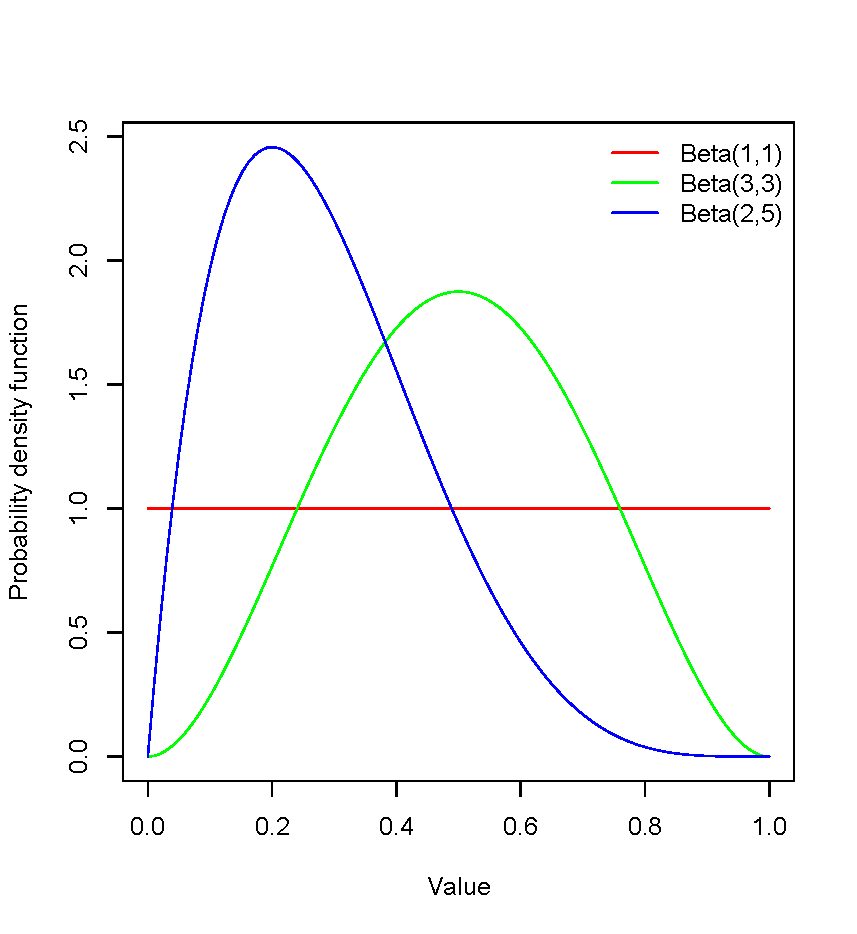
\includegraphics[width=0.5\textwidth]{betas.pdf}
\end{center}

\subsection*{Analysis of distributions}
\begin{enumerate}
\item
$Beta(1,1)$: this Beta is just the uniform distribution on the $(0,1)$ interval, which can be interpreted as the ratio of wins and losses in the past being uniformly distributed in the $(0,1)$ interval.
\item
$Beta(3,3)$: this distribution prefers ratio of wins and losses concentrated around $0.5$, meaning that the number of wins and losses that have been observed in the past are fairly similar.
\item
$Beta(2,5)$: finally, this Beta prefers low ratio of wins and losses, which can be interpreted as more losses than wins have being observed in the past.
\end{enumerate}

\item % 2e

For the MAP estimation, we want to find:
$$\theta_{MAP}=arg\max_{\theta}{p(\Theta=\theta\ |\mathcal D)}$$
The very useful property of the Beta distribute is that the maximum $p(\Theta=\theta)=Beta(\Theta=\theta|\alpha,\beta)$ can be easily calculated as $\frac{\alpha-1}{\alpha+\beta-2}$, so we can easily find the MAP estimate for $\theta$ as:

$$\theta_{MAP}=\frac{\alpha+N_1-1}{\alpha+\beta+N-2}$$

Where $N_1$ is the number of wins, and $N$ is the total of matches.

\item % 2f
Using data from \texttt{http://www.gocrimson.com/sports/fball/2011-12/schedule}, we can see that Harvard lost its first game, and won all the others $9$ in the $2011$-$2012$ season. This is going to be our prior distribution. Also, Harvard won all the three first games of this season.

\begin{enumerate}[i.]
\item
\textbf{Maximum likelihood}
$$p(\bm{x} = 1|\mathcal D)=arg\max_\theta{p(\mathcal D|\bm{\theta}})$$
$$p(\mathcal D|\bm{x}=1)=\frac{3}{3}=1$$
$$p(\mathcal D|\bm{x}=0)=\frac{0}{3}=0$$

Thus, we predict that the probability that the team will win is $p(\bm{x}=1|\mathcal D)= 1$.

\item
\textbf{Maximum a posteriori}:
$$\theta_{MAP}=\frac{\alpha+N_1-1}{\alpha+\beta+N-2}$$
For the Beta, we will have $\alpha=9$ and $\beta=1$, so:
$$\theta_{MAP}=\frac{9+3-1}{9+1+3-2}=\frac{13}{13}=1$$

Thus, we predict that the probability that the team will win is $p(\bm{x}=1|\mathcal D)=1$.
\item
\textbf{Full Bayesian}: the predictive distribution for the new datum will be:
$$p(\bm{x}=1|\mathcal D)= \int_\Theta P(\bm{x}|\theta)P(\theta | \mathcal{D})\,d\theta=\int_0^1 P(\bm{x}=1|\theta)P(\theta | \mathcal{D})\,d\theta$$
$$p(\bm{x}=1|\mathcal D)= \frac{\alpha+N_1}{\alpha+\beta+N}=\frac{9+3}{10+3}\approx 0.923$$
Thus, we predict that the probability that the team will win is $p(\bm{x}=1|\mathcal D)\approx 0.923$.

\end{enumerate}

\end{enumerate}

\section*{Problem 3}

\begin{enumerate}[a.]

\item % 3a

% ANSWER FOR 3A HERE

\item % 3b

% ANSWER FOR 3B HERE

\end{enumerate}
\newpage
\section*{Problem 4}

\begin{enumerate}[a.]


\item % 4a

% ANSWER FOR 4AA HERE
\newpage
\item % 4ab

% ANSWER FOR 4AB HERE
\begin{enumerate}[(a)]

\item % 4ba
Using the $min$ and $max$ distance metrics:\\

\begin{center}
       \begin{tabular}{|c|c|c|} \hline
           & Number of instances for $min$ & Number of instances for $max$\\ \hline
            \verb|Cluster 1| & \verb|73| & \verb|19|\\ \hline
            \verb|Cluster 2| & \verb|25| & \verb|23|\\ \hline
            \verb|Cluster 3| & \verb|1| & \verb|32|\\ \hline
            \verb|Cluster 4| & \verb|1| & \verb|26|\\ \hline
        \end{tabular}

\end{center}
\begin{figure}[htb]
\begin{center}
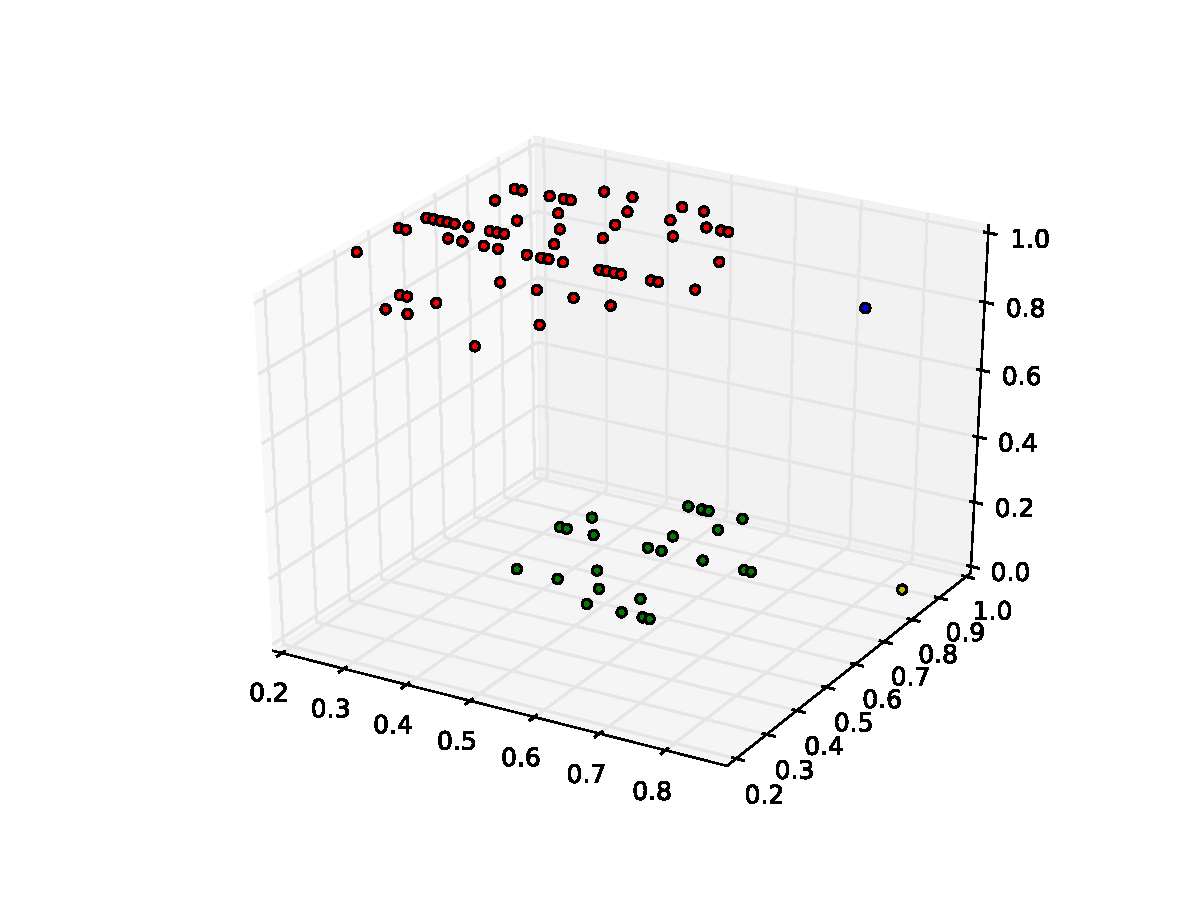
\includegraphics[width=0.45\textwidth]{3dplot_4_100_min.pdf}
\caption{$min$ distance metric}
\end{center}
\end{figure}

\begin{figure}[htb]
\begin{center}
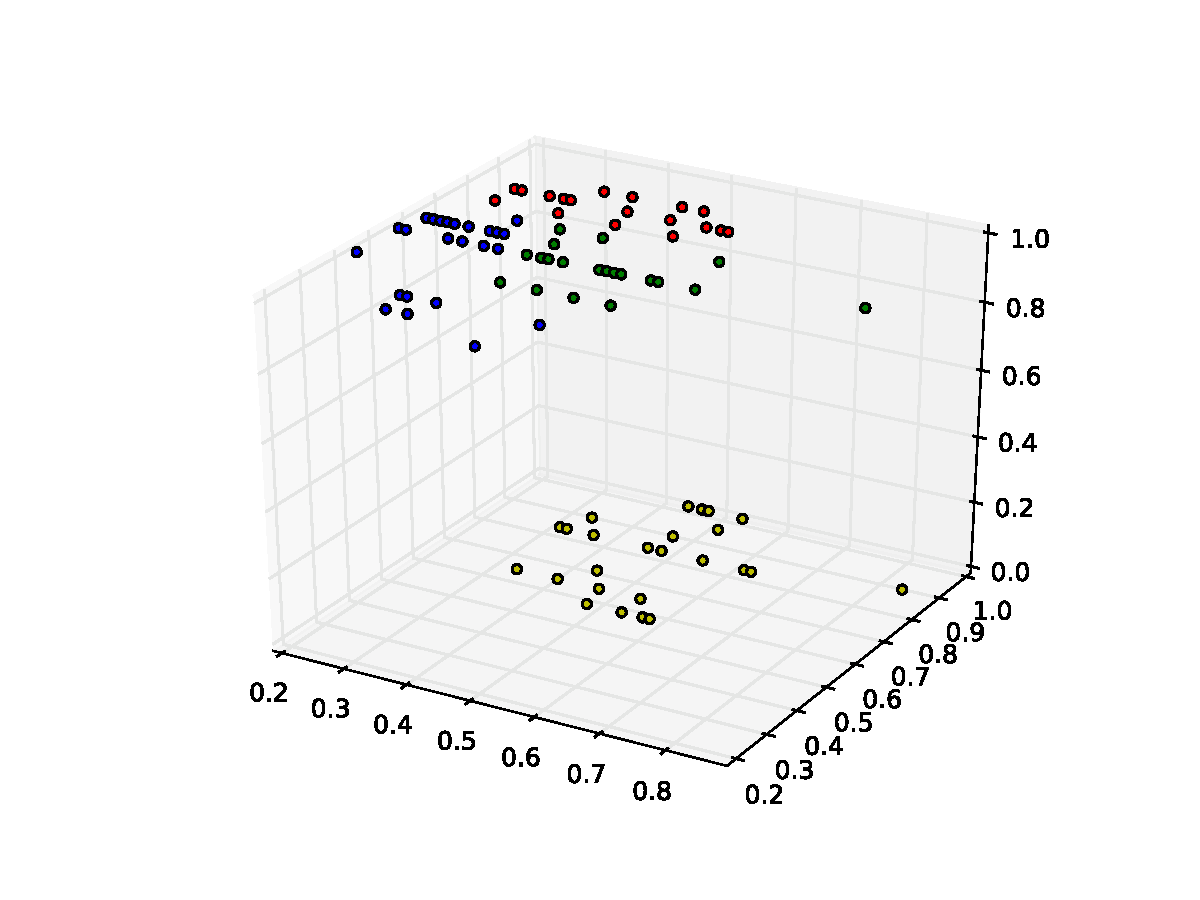
\includegraphics[width=0.45\textwidth]{3dplot_4_100_max.pdf}
\caption{$max$ distance metric}
\end{center}
\end{figure}

\subsection*{Analysis}
The $min$ distance metric seems to be very good at clustering fairly  evident chunks of data that at a nearby regions in space, so the result of that are clusters isolating four very distinct and spaced blobs. The downside of that, however, is that specially isolated data doesn't get merged to other clusters, which makes HAC merge important and different clusters in order to preserve the isolated cluster that fails to get merged with any other cluster. As an example, if we had three points in space very isolated from any other points and from each other, they would each be a different cluster, and all the other points would be the forth (and gigantic) cluster of the output. That would not be very helpful, since the big chunk of data that we want to classify is basically not even being separated because the $min$ metric doesn't respond well to noisy data like that. Those properties totally make sense based on the $min$ distance metric - isolated points would have such large distances to any other points that they would hardly be able to be merged to any other clusters.\\

The $max$ metric, on the other hand, is much better at dealing with noise. We can see that both of the isolated points in space got merged to another fairly close cluster, making the isolation of the data on the upper left of the graph more specific, and leading to three different clusters on the top, as opposed to the single one when using $min$. The disadvantage of that is that maybe the breaks that $max$ did on the top cluster are not even that clear, and maybe not even appropriate. There clearly is a tradeoff between $min$ and $max$, and there is no right answer on which one would be better for a generic classification problem. When developing clustering for some data using HAC, it would be appropriate to test the clustering on some training data using different types of distance metric, to be sure to choose the most appropriate one for the kind of data we are dealing with. The properties observed also make sense according to the $max$ distance metric - the algorithm will be sure to merge isolated (and possible noisy) clusters so that their noise don't compromise the overall algorithm performance.

\newpage
\item % 4bb

Using the $mean$ and $centroid$ distance metrics:\\

\begin{center}
       \begin{tabular}{|c|c|c|} \hline
           & Number of instances for $mean$ & Number of instances for $centroid$\\ \hline
            \verb|Cluster 1| & \verb|143| & \verb|147|\\ \hline
            \verb|Cluster 2| & \verb|9| & \verb|47|\\ \hline
            \verb|Cluster 3| & \verb|47| & \verb|5|\\ \hline
            \verb|Cluster 4| & \verb|1| & \verb|1|\\ \hline
        \end{tabular}

\end{center}
\begin{figure}[htb]
\begin{center}
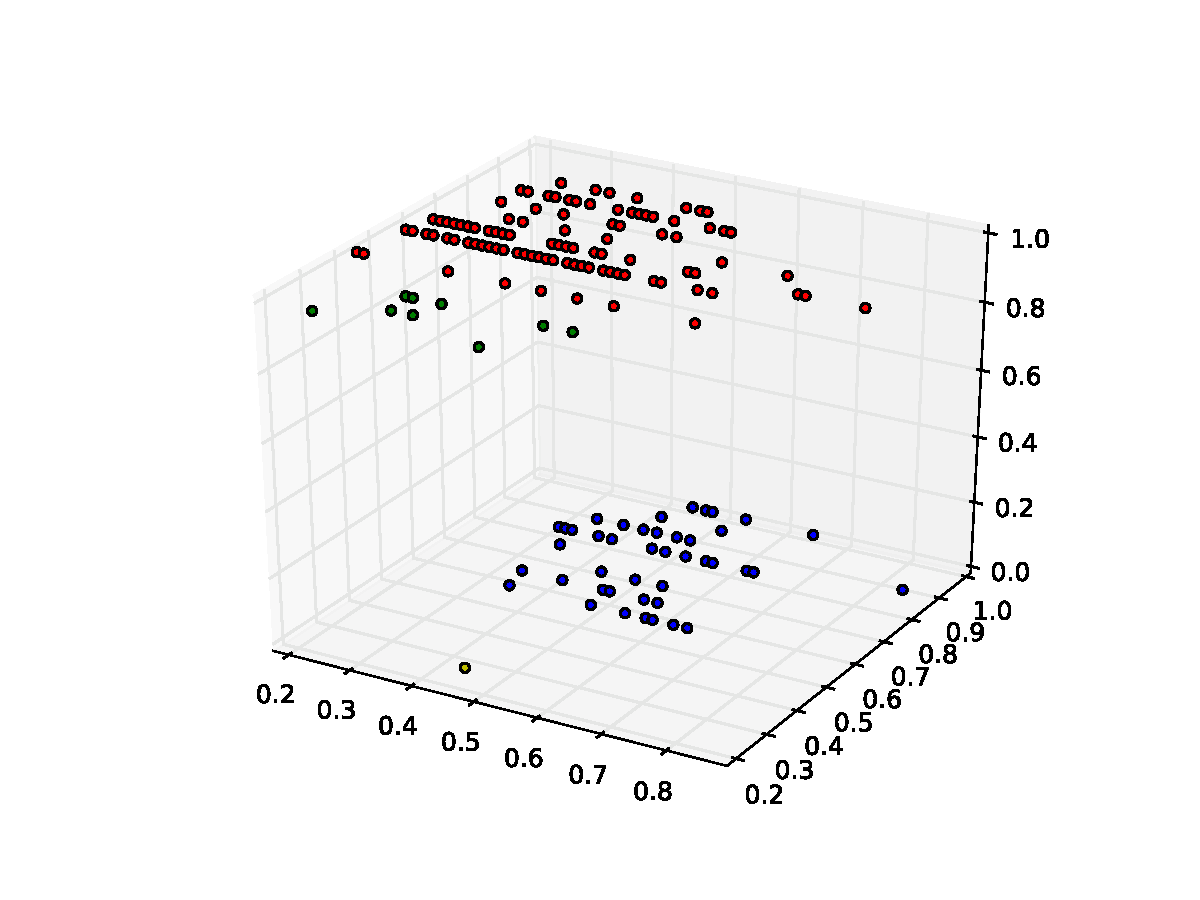
\includegraphics[width=0.45\textwidth]{3dplot_4_200_mean.pdf}
\caption{$mean$ distance metric}
\end{center}
\end{figure}

\begin{figure}[htb]
\begin{center}
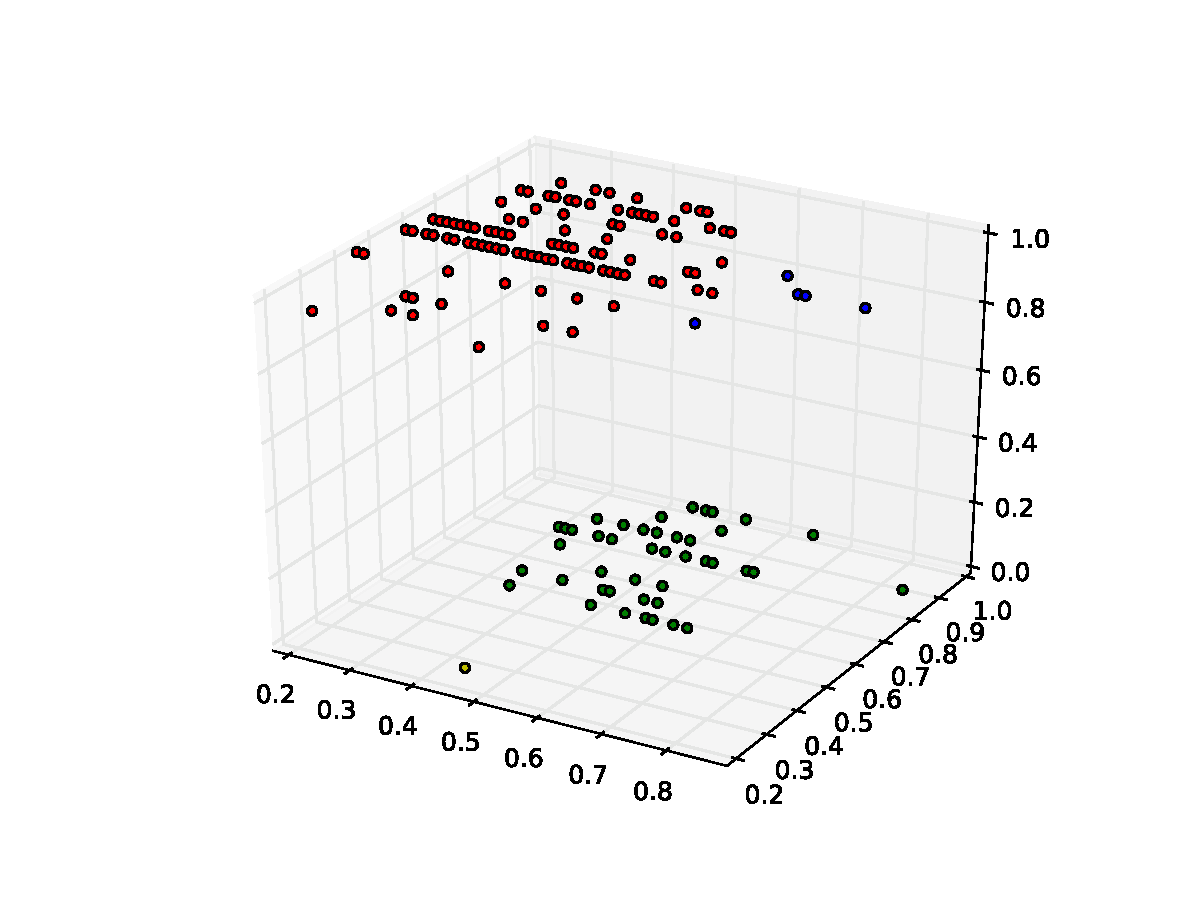
\includegraphics[width=0.45\textwidth]{3dplot_4_200_cent.pdf}
\caption{$centroid$ distance metric}
\end{center}
\end{figure}

\end{enumerate}
\subsection*{Analysis}
The $mean$ distance metric seems to be good at clustering chunks of data with small variances, as would be expected from a method that uses averages for deciding on clustering. Since the metric uses all points in a cluster to decide on merging clusters, the method seems to be less susceptible to being biased by very extreme values, although we do see a cluster with only one very isolated element in it, which shows that the metric is still not perfect at avoiding such bias.\\

The $centroid$ distance metric seems to perform equally to $mean$ for the bottom clusters, but the clustering behavior is very different for the two top ones. It is easy to see that the red cluster has a centroid on the upper left, while the blue one has a centroid on the right, which shows that the principle of the metric is being followed. Since $centroid$ distance metric takes all points in consideration for clustering, outliners don't have a very significant effect on its performance. Still, the method didn't seem to find very interesting clusters except for the obvious red and green ones, which suggests that extreme values are still an issue for such method.

\newpage

\item 

\begin{enumerate}[(a)]

\item % 4ca

% ANSWER FOR 4CA HERE

\item % 4cb

% ANSWER FOR 4CB HERE

\item % 4cc

% ANSWER FOR 4CC HERE

\end{enumerate}

\end{enumerate}

\end{document}